%% V1.0
%% by Gabriel Garcia, gabrcg@gmail.com
%% This is a template for Udacity projects using IEEEtran.cls

%% Be Udacious!

\documentclass[10pt,journal,compsoc]{IEEEtran}

\usepackage[pdftex]{graphicx}    
\usepackage{cite}
\hyphenation{op-tical net-works semi-conduc-tor}


\begin{document}

\title{Robotic Inference}

\author{Seyfi Gozubuyuk}

\markboth{Inference project, Robotic Nanodegree, Udacity}%
{}
\IEEEtitleabstractindextext{%

\begin{abstract}
Deep Learning is widely used in object classification. Convolutional Neural Networks improved the success of the computers on object detection, recognition and classification. They are widely used in Self-Driving Cars, robotics and bla bla 
There exist models such as LeNet, AlexNet, and GoogleNet. Nvidia Digits provides a web interface to utilize these models and create other models.  It is possible to upload data and test it with these models. This project includes to different classification tasks on image datasets. 

TODO DELETE
In this project, the aim is to train a Deep Neural Network to classify the images of different objects. Nvidia Digits is the main tool for the project. 

An abstract is meant to be a summary of all of the relevant points in your presented work. It is designed to present a high-level overview of the report, providing just enough detail to convey the necessary information The abstract may often mention a one-sentence summary of the results.  While the type of voice chosen for the paper (active or passive) may be up for debate, you should avoid the use of “I” and “me” in the report. It usually is kept to a length of 150 - 200 words. 
Example: You should not write, “I present two different neural networks for classifying my data”. Instead, you should try to say, “Two different neural networks are used for classification”.
TODO DELETE
\end{abstract}

% Note that keywords are not normally used for peerreview papers.
\begin{IEEEkeywords}
Robot, IEEEtran, Udacity, \LaTeX, Deep Learning, Convolutional Neural Networks, Nvidia Digits.
\end{IEEEkeywords}}


\maketitle
\IEEEdisplaynontitleabstractindextext
\IEEEpeerreviewmaketitle
\section{Introduction}
\label{sec:introduction}

\IEEEPARstart{T}{he} goal in this project is to utilize Nvidia Digits application to perform classification on image datasets. There are two datasets. The first one is the provided data that contains bottle and candy box images. Besides, there exists image that do not contain any. 

TODO The second dataset.

Nvidia Digits provide an interface to load the data, create a new model or utilize predefined models. In addition, it enables to customize the models and select hyper parameters. During training, it saves the model on every epoch. This saved models can be used as pretrained models to train more.


% TODO DELETE
% introduction should provide some material regarding the history of the problem, why it is important and what is intended to be achieved. If there exists any previous attempts to solve this problem, this is a great place to note these while conveying the differences in your approach (if any). The intent is to provide enough information for the reader to understand why this problem is interesting and setting up the conversation for the solution you have provided
% Use this space to introduce your robotic inference idea and how you wish to apply it. 
% If you have any papers / sites you have referenced for your idea, please make sure to cite them.

% %example for inserting image
% \begin{figure}[thpb]
%       \centering
%       \includegraphics[width=\linewidth]{RobotRevolution5}
%       \caption{Robot Revolution.}
%       \label{fig:robot1}
% \end{figure}

% \subsection{Subsection Heading Here}
% Subsection text here.

% \subsubsection{Subsubsection Heading Here}
% Subsubsection text here.


% \begin{table}[h]
% \caption{Table}
% \label{table_example}
% \begin{center}
% \begin{tabular}{|c||c|}
% \hline
% One & Two\\
% \hline
% Three & Four\\
% \hline
% \end{tabular}
% \end{center}
% \end{table}
% TODO DELETE


   

\section{Background / Formulation}
The problem is to classify objects using Deep Learning. Convolutional neural networks are a good choise\cite{wiki:cnn}. Backpropagation provided enhanced learning for Multilayer Neural Networks.

\subsection{LeNet}
LeCun et al., 1998 developed LeNet to classify digits in 1998\cite{lenet}. LeNet is a seven level CNN.

\subsection{AlexNet}
AlexNet\cite{AlexNet}

\subsection{GoogleNet}
GoogleNet\cite{gnet}

\subsection{Task 1: Bottle vs Candy-Box}
In the first task, AlexNet and GoogleNet were selected to classify the samples of bottles and candy-boxes. The reason for selecting AlexNet is its speed, and the reason for selecting the GoogleNet was its higher accuracy. Five different models trained during completing this task. Since adam and RMSprop helps the gradient descent to reach the minima faster, these solver types were allied with AlexNet and GoogleNet. Besides the Stochastic Gradient Descent were selected with AlexNet as the default option. Learning rate 0.01 was a reasonable choise to prevent overfitting and overshooting. The image sizes were compatible with AlexNet and GoogleNet, therefore there were no changes on sizes. Different number of epochs were tried. The results section discuss the details of the models tried and the outcomes.


% TODO DELETE
% LeNet
% AlexNet
% GoogleNet
% SGD, adam, RMSprop
% TODO DELETE

\subsection{Task 2: TODO}

% TODO DELETE
% At this stage, you should begin diving into the technical details of your approach by explaining to the reader how parameters were defined, what type of network was chosen, and the reasons these items were performed. This should be factual and authoritative, meaning you should not use language such as “I think this will work” or “Maybe a network with this architecture is better..”. Instead, focus on items similar to, ”A 3-layer network architecture was chosen with X, Y, and Z parameters” 
% Explain why you chose the network you did for the supplied data set and then why you chose the network used for your robotic inference project.

% %example for Bullet point list

% \begin{itemize}
% \item example
% \end {itemize}



% %example for numbered list
% \begin{enumerate}
% \item example

% \end{enumerate}
% TODO DELETE


\section{Data Acquisition}
The first task does not contain any changes on the data, since the models were compatible with image size of 256x256.

TODO SECOND TASK

This section should discuss the data set. Items to include are the number of images, size of the images, the types of images (RGB, Grayscale, etc.), how these images were collected (including the method). Providing this information is critical if anyone would like to replicate your results. After all, the intent of reports such as these are to convey information and build upon ideas so you want to ensure others can validate your process.
Justifying why you gathered data in this way is a helpful point, but sometimes this may be omitted here if the problem has been stated clearly in the introduction.
It is a great idea here to have at least one or two images showing what your data looks like for the reader to visualize.

\section{Results}
\subsection{Task 1: Bottle vs Candy-Box}
The results for the five different model for the Task 1 are given on Table~\ref{table:t1r}.

\begin{table}[h]
\caption{Results on Task 1}
\label{table:t1r}
\begin{center}
\begin{tabular}{|c||c||c||c||c||c||c|}
\hline
No. & Model & Epoc & Solver & Rate & Accuracy \\
\hline
1* & AlexNet1 & 30 & RSMprop & 0.01 & 73.77\%\\
\hline
2* & AlexNet1E17 & 5 & RSMprop & 0.0001 & 70.49\%\\
\hline
3 & GoogleNet & 6 & Adam & 0.01 & 67.21\%\\
\hline
4* & GoogleNetE6 & 4 & Adam & 0.01 & 67.21\%\\
\hline
5 & AlexNet2 & 10 & SGD & 0.01 & 75.41\%\\
\hline
\end{tabular}
\end{center}
1* RMS decay value for 1.AlexNet1 and 2.AlexNet1E17 were 0.99\\
2* AlexNet1E17 started from the Epoch 17 of model 1.AlexNet1\\
4* GoogleNetE6 started from the Epoch 6 of model 3.GoogleNet
\end{table}

Figures~\ref{fig:t1a2c} shows the screenshot of the console when evaluating the AlexNet2 model for Task1.

TODO ADD FIGURES
\begin{figure}[thpb]
      \centering
      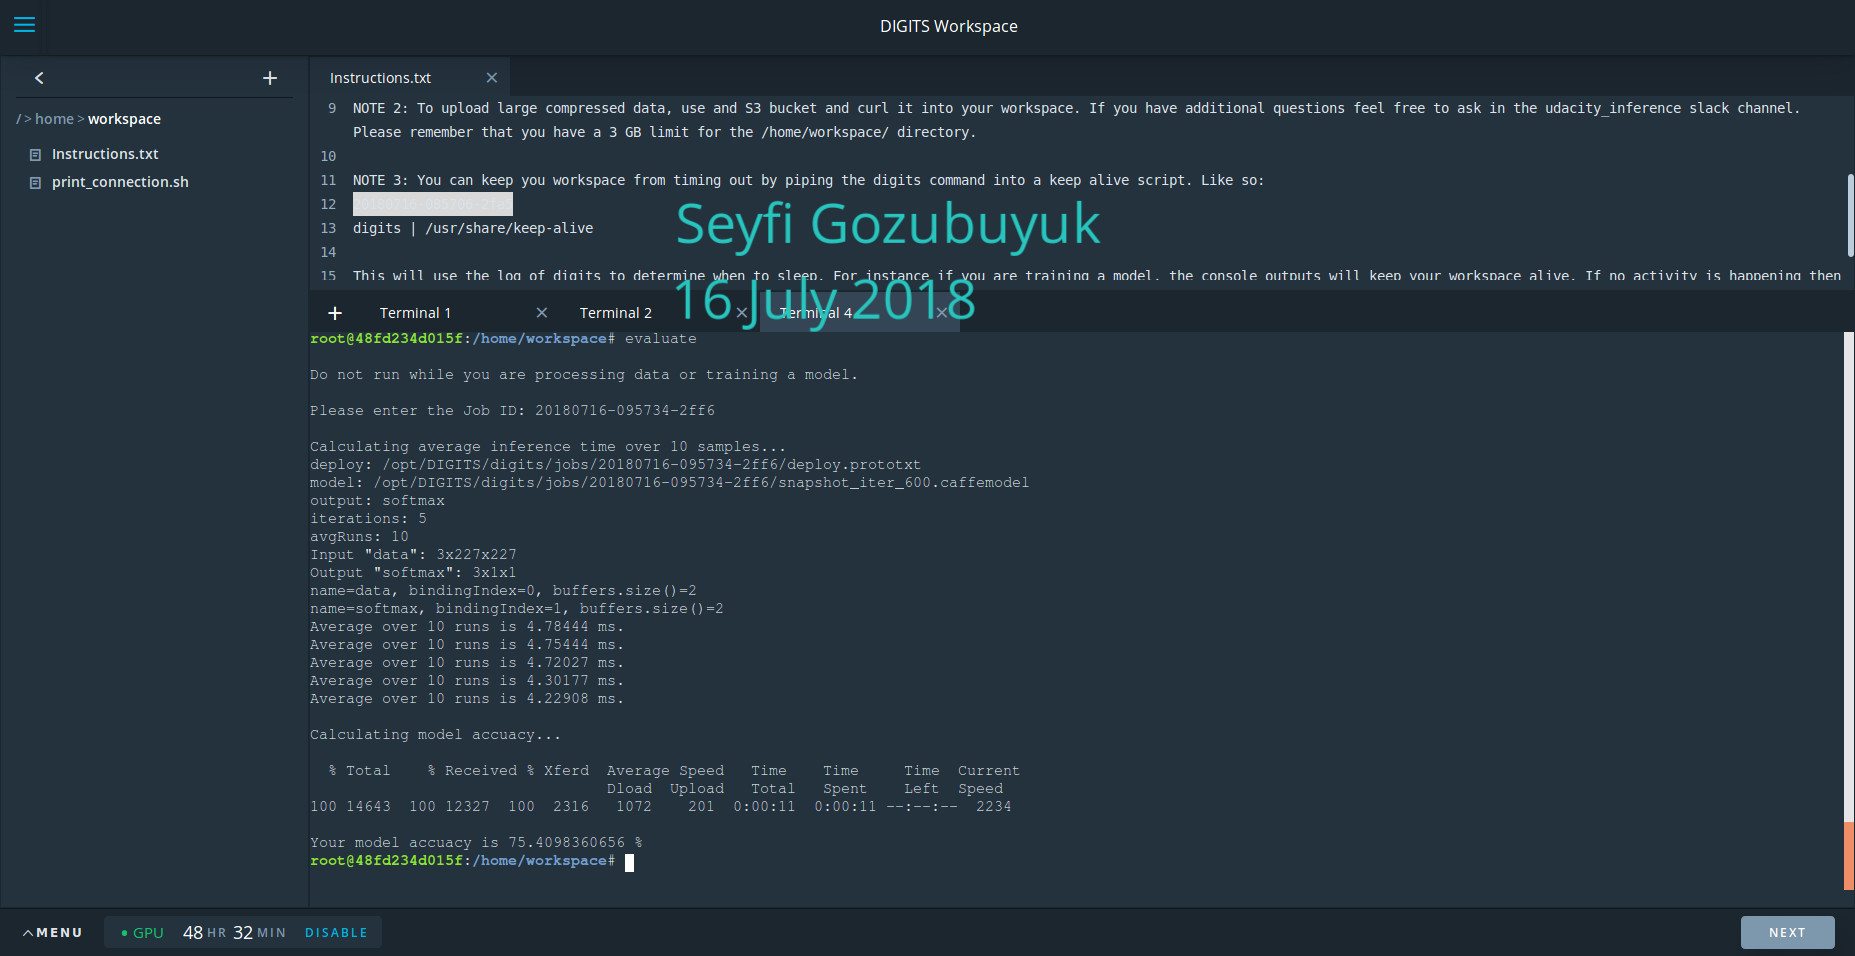
\includegraphics[width=\linewidth]{figures/t1a2c.png}
      \caption{Screenshot of Task 1 AlexNet2}
      \label{fig:t1a2c}
\end{figure}

Figures~\ref{fig:t1a2g} shows the training graph of successful AlexNet2 model. Figures~\ref{fig:t1a2l}, Figures~\ref{fig:t1a2t1}, Figures~\ref{fig:t1a2t2}, and Figures~\ref{fig:t1a2t3} shows the classification results of testing AlexNet2.

\begin{figure}[thpb]
      \centering
      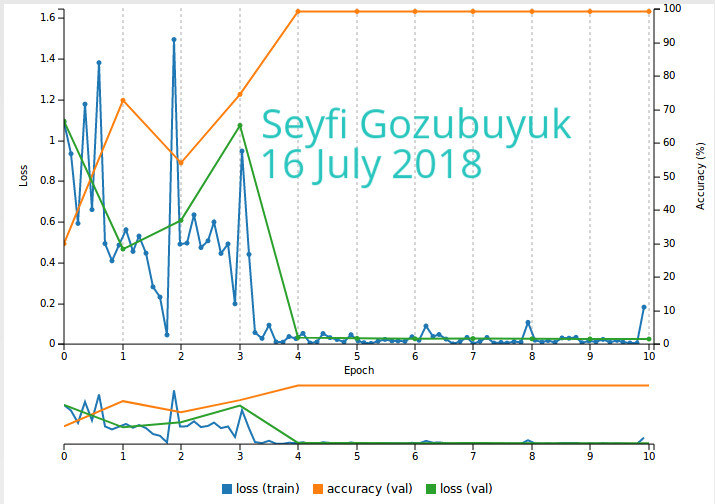
\includegraphics[width=\linewidth]{figures/t1a2g.png}
      \caption{Training Graph of Task 1 AlexNet2}
      \label{fig:t1a2g}
\end{figure}

\begin{figure}[thpb]
      \centering
      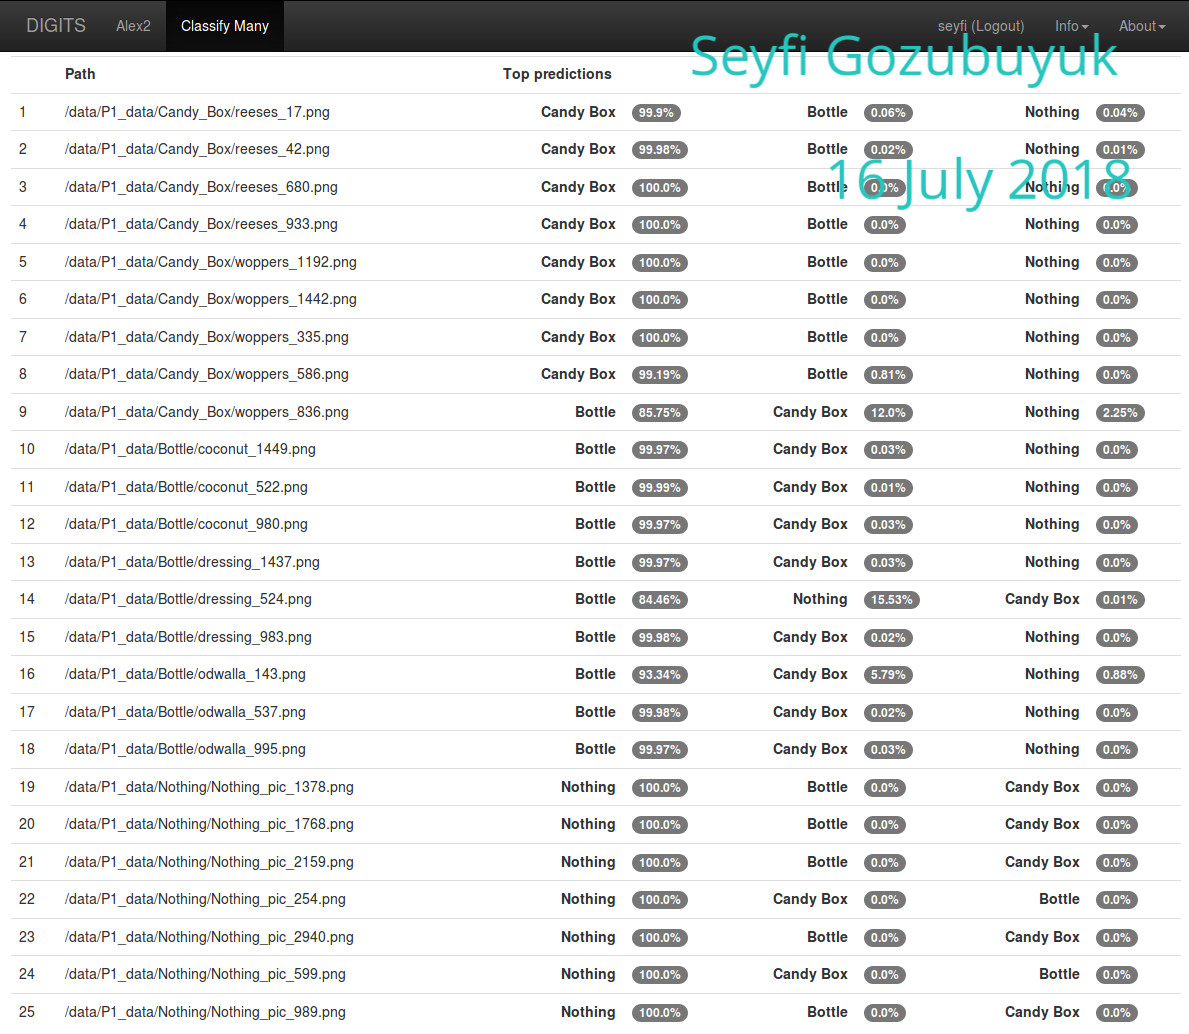
\includegraphics[width=\linewidth]{figures/t1a2l.png}
      \caption{Testing 25 Images with Task 1 AlexNet2}
      \label{fig:t1a2l}
\end{figure}


\begin{figure}[thpb]
      \centering
      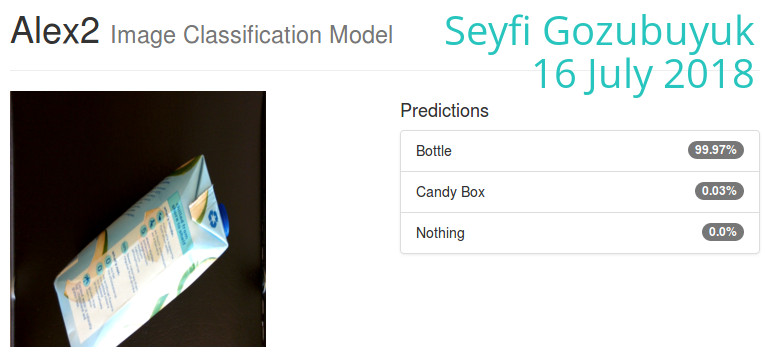
\includegraphics[width=\linewidth]{figures/t1a2t1.png}
      \caption{Testing a Bottle Image Task 1 AlexNet2}
      \label{fig:t1a2t1}
\end{figure}


\begin{figure}[thpb]
      \centering
      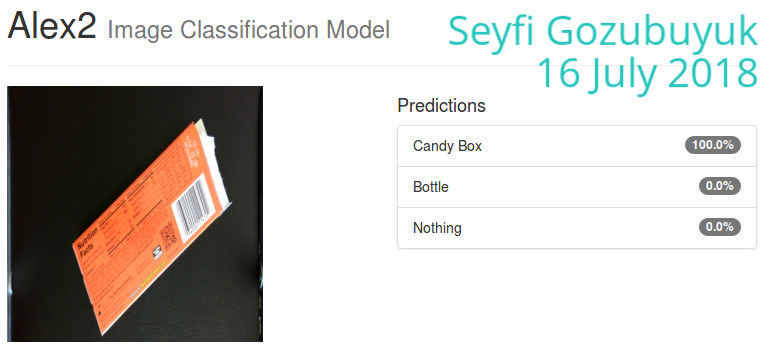
\includegraphics[width=\linewidth]{figures/t1a2t2.png}
      \caption{Testing a Candy-Box Image Task 1 AlexNet2}
      \label{fig:t1a2t2}
\end{figure}


\begin{figure}[thpb]
      \centering
      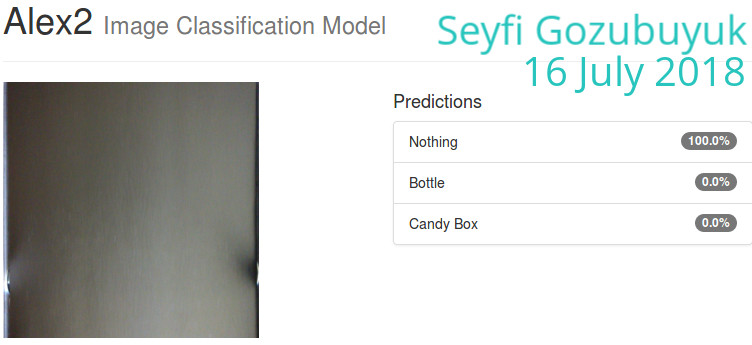
\includegraphics[width=\linewidth]{figures/t1a2t3.png}
      \caption{Testing a Nothing Image Task 1 AlexNet2}
      \label{fig:t1a2t3}
\end{figure}



Figures~\ref{fig:t1a1g} shows the training graph of unsuccessful AlexNet1 model. The accuracy graph shows that the highest accuracy was obtained at epoch 17.

\begin{figure}[thpb]
      \centering
      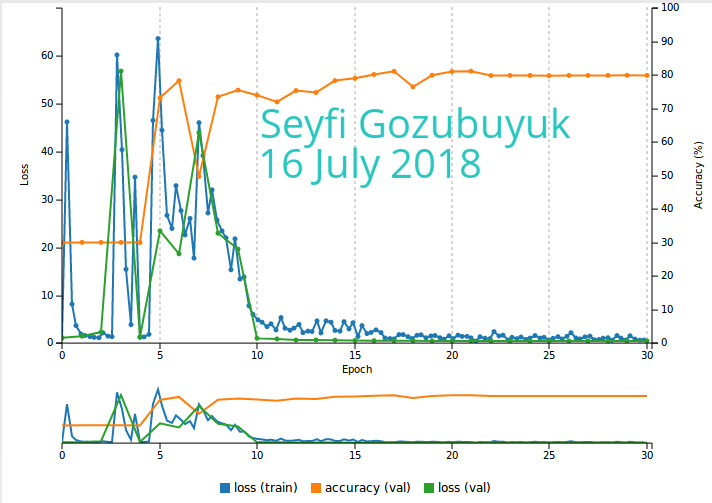
\includegraphics[width=\linewidth]{figures/t1a1g.png}
      \caption{Training Graph of Task 1 AlexNet1}
      \label{fig:t1a1g}
\end{figure}


TODO SECOND SECTION
\subsection{Task 1: Bottle vs Candy-Box}

This is typically the hardest part of the report for many. You want to convey your results in an unbiased fashion. If you results are good, you can objectively note this. Similarly, you may do this if they are bad as well. You do not want to justify your results here with discussion; this is a topic for the next session. 
Present the results of your robotics project model and the model you used for the supplied data with the appropriate accuracy and inference time
For demonstrating your results, it is incredibly useful to have some charts, tables, and/or graphs for the reader to review. This makes ingesting the information quicker and easier.

\section{Discussion}
The graph ... shows that SGD worked better on the dataset. 

This is the only section of the report where you may include your opinion. However, make sure your opinion is based on facts. If your results are poor, make mention of what may be the underlying issues. If the results are good, why do you think this is the case? Again, avoid writing in the first person (i.e. Do not use words like “I” or “me”). If you really find yourself struggling to avoid the word “I” or “me”; sometimes, this can be avoid with the use of the word “one”. As an example: instead of : “I think the accuracy on my dataset is low because the images are too small to show the necessary detail” try: “one may believe the accuracy on the dataset is low because the images are too small to show the necessary detail”. They say the same thing, but the second avoids the first person. 
Reflect on which is more important, inference time or accuracy, in regards to your robotic inference project.

\section{Conclusion / Future work}
This section is intended to summarize your report. Your summary should include a recap of the results, did this project achieve what you attempted, and is this a commercially viable product? 
For Future work,address areas of work that you may not have addressed in your report as possible next steps. For future work, this could be due to time constraints, lack of currently developed methods / technology, and areas of application outside of your current implementation. Again, avoid the use of the first-person.

\bibliography{bib}
\bibliographystyle{ieeetr}

\end{document}